\section{Experimental Parameters}
Useful output parameters and input parameters were defined in order to carry out the series of comparative constellation studies. The output parameters from the STK model were used in order to quantify the relationship between constellation input parameters and system performance.
\subsection{Performance Metrics}
\label{sec:perfMetrics}
ADS-B coverage for a each satellite constellation was analysed on a flight-by-flight basis. For a given constellation, the communication link was analysed separately for a sample of trans-oceanic test flights. Each link was characterised by three parameters -
\begin{itemize}
	\item \textbf{Access Times} - the periods of time during which a flight had line-of-sight to at least one overhead satellite and therefore could theoretically establish an ADS-B link. This was available as primary data from STK.
	\item \textbf{Coverage Gap Times} - the periods of time during which a flight has line-of-sight access to no satellites in the constellation. This was calculated after evaluating data from STK.
	\item \textbf{Received Isotropic Power} - the power of the ADS-B signal after it has been propagated from a flight to an overhead satellite. This was available as primary data from STK \footnote{Although the STK communication toolkit was capable of RF link characterisation beyond simply received isotropic power, it was found that the `simple' antenna models used were not adequate for that level of analysis. The results, typified by Table \ref{tab:results_linkbudget_sample1}, show a very high bit-error rate and bad signal-to-noise ratio. The values were such that the development of a signal processing module would be near impossible. A more realistic set of signal characteristics could be achieved by more sophisticated antenna and RF models. However the knowledge required to design the model was beyond the scope of this thesis. Instead, we simply used received power as a comparative indicator of RF performance of the system.}.
\end{itemize}

 
From this data, four values were computed and used as performance metrics to evaluate the efficacy of a constellation - 
\begin{enumerate}
	\item \textbf{Total coverage gap fraction} - the fraction of time a simulated flight spends without being able to transmit ADS-B signals to a satellite. This would be representative of the time the flight would expect to spend out of communication for a given period of time. This was calculated by the formula
	\[ \dfrac{\text{total time with no access to a satellite}}{\text{total analysis time}}\]
	\item \textbf{Maximum gap time} - the maximum amount of time a flight spends without a communication link to a satellite. This represents the worst case scenario for the amount of time a flight would spend out of communication.
	\item \textbf{Average Gap Time} and \textbf{Average Access Time} - the mean of access times and coverage gap times identified during the analysis period. This would give an indication of the periodicity of the 'access-no access' cycles that a flight would experience.
	\item \textbf{Minimum Received Isotropic Power} - the minimum power of an ADS-B signal as it is received by a satellite. This can be used to later determine the link budgets and perform the system definition for a given satellite in the constellation.
	
\end{enumerate}
The relative importance of these performance metrics will be compared in section \ref{sec:decision_matrix}

\subsection{Flight Selection} \label{sec:flight_selection}
OpenFlights \cite{Open} has statistics on all flight paths currently being serviced by major airlines, illustrated in Figure \ref{fig:flightpaths}.
\begin{figure}[htbpp]
	\centering
	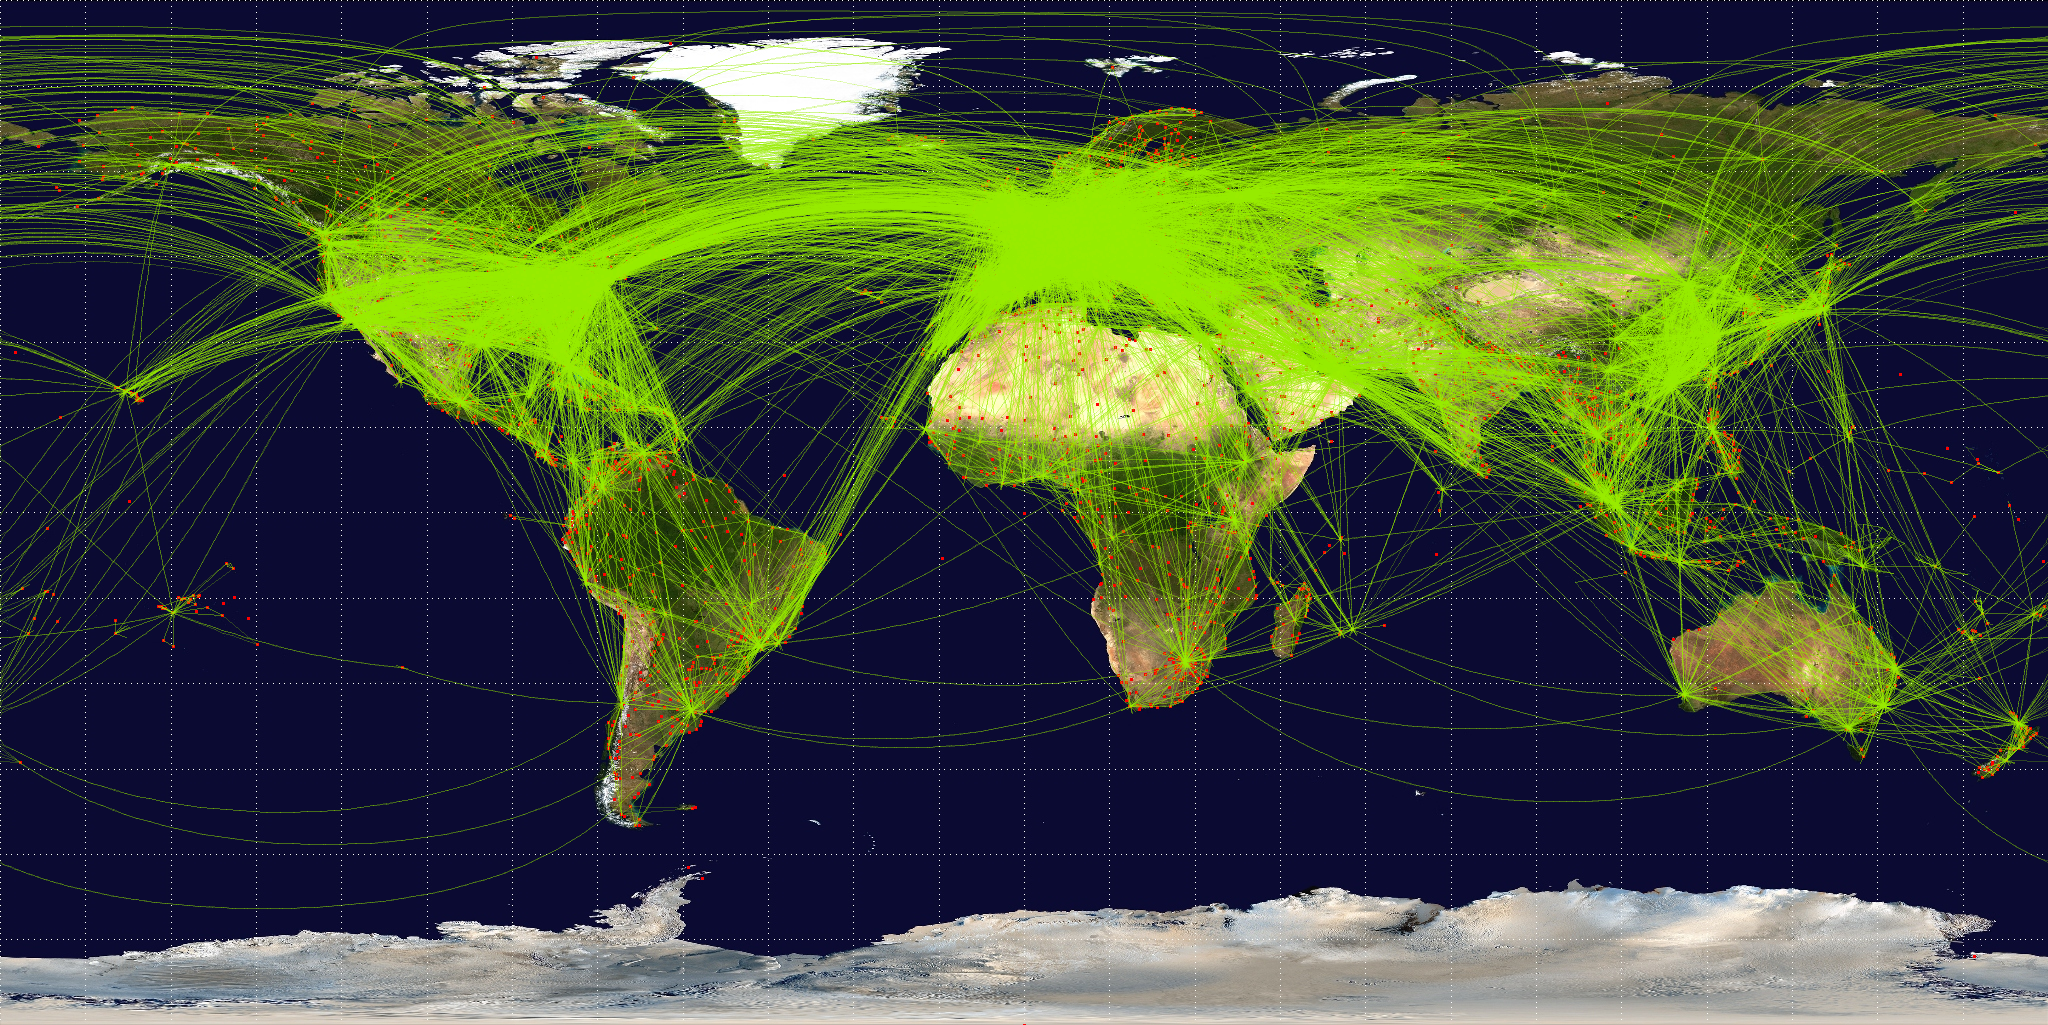
\includegraphics[scale = 0.18]{Pictures/flightpaths.png}
	
	\caption[Popular flight routes]{Popular flight routes, from \cite{Open}}
	\label{fig:flightpaths}
\end{figure} 

The advantages of space-based ADS-B coverage would mainly come from areas where ground-coverage is not possible. For this reason, flight paths that were primarily over land-masses were not considered for analysis. This eliminated the majority of flights originating in the EU and ending in any of Africa, Asia and Australia. Analysis then focussed on flights passing over the Atlantic and Pacific Oceans. These flights were mostly between the United States and Europe, Asia and Australia, as shown in Figure \ref{fig:transoceanicflights}.

\begin{figure}[H]
	\centering
	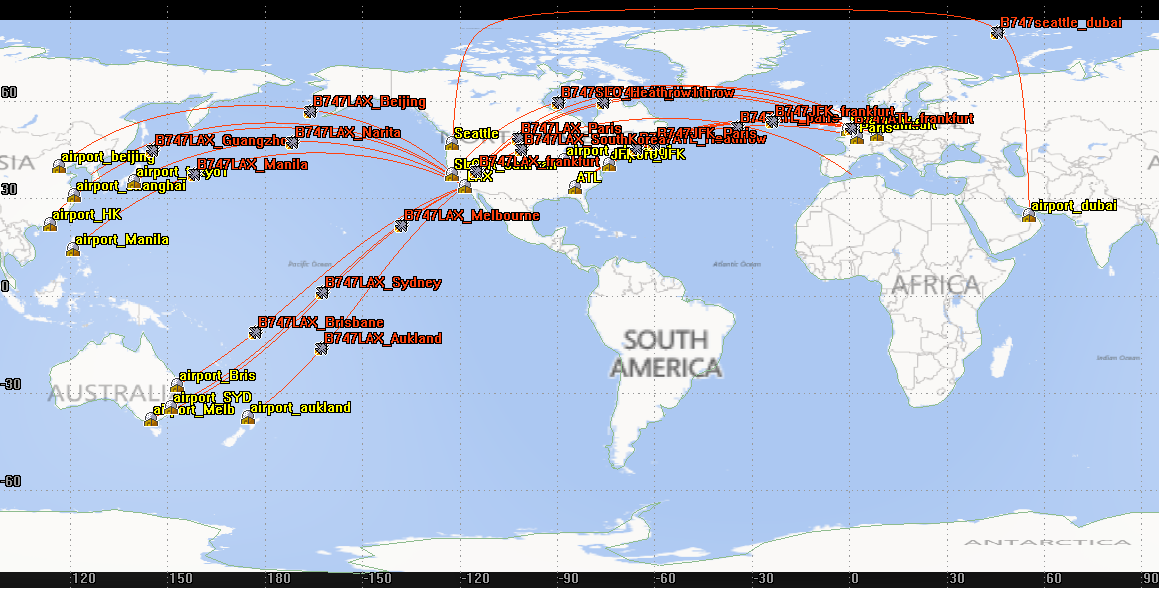
\includegraphics[scale = 0.45]{Pictures/transoceanicflights.png}
	
	\caption{Trans-Oceanic Flight paths, as modelled in STK}
	\label{fig:transoceanicflights}
\end{figure} 

Of these flights, three generalisations were defined and one flight from each generalisation was used for modelling -
\begin{enumerate}
	\item \textbf{North America to Asia} - The path between Los Angeles International Airport (LAX) and Narita airport (NRT) in Tokyo Japan 
	\item \textbf{North America to Europe} - The path between LAX and Heathrow (LHR).
	\item \textbf{North America to Australia} - The path between LAX and Sydney (SYD) International Airport.
\end{enumerate}
These generalisations are highlighted in red Figure \ref{fig:transoceanicGeneralisations}.


\begin{figure}[H]
	\centering
	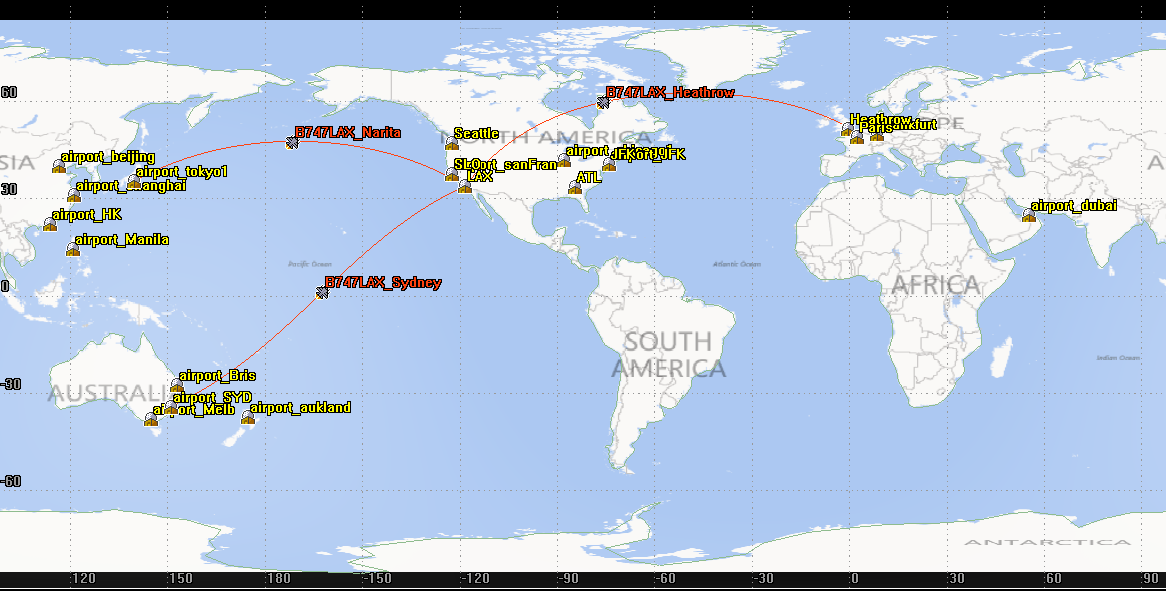
\includegraphics[scale = 0.55]{Pictures/transoceanicGeneralisations.png}
	
	\caption{Generalisations of trans-Oceanic Flight paths used for analysis}
	\label{fig:transoceanicGeneralisations}
\end{figure} 

The performance of a given constellation was determined by examining the ADS-B coverage available for each flight by the parameters outlined in Section \ref{sec:perfMetrics}. The flights were simulated as going continuously back and forth between their two destination airports. The effect of this periodicity is expanded upon in Section \ref{sec:analysis_period}.

\subsection{Input Variables}
The performance metrics presented in Section \ref{sec:perfMetrics} were evaluated against different constellation configurations. Initial tests, discussed later in Section \ref{sec:initial_constel}, ruled out Molniya, geostationary and medium to high earth orbits as practical solutions. The parametric study was then restricted to Low-Earth Orbits, varying orbital parameters from a `reference case'.

\subsubsection{Reference Case} \label{sec:ref_case}
The reference case was chosen to be a constellation of 12 satellites distributed in three circular orbital planes, each with four equispaced satellites. Each orbital plane was inclined at 60 degrees and were at an altitude of 700km above the Earth (a semi-major axis of 7078.14km). The three planes were separated by 120 degrees of Right Angle of Ascending Node (RAAN), starting from 0 degrees for plane one. The four satellites within each plane were separated by true anomalies of 90 degrees. These parameters are summarised in Table \ref{tab:satRefCase}. The ground track of the configuration is shown in Figure \ref{fig:12sat_2d} and the 3D representation is given in Figure \ref{fig:12sat_3d}

\begin{table}[htbp]
  \centering
  \caption{`Reference' constellation configuration}
    \begin{tabular}{lr}
    \toprule
    Parameter & Value\\
    \midrule
    Total number of satellites & 12  \\
    Orbital planes	& 3\\
    Satellites per plane & 4\\
    Separation between planes & 120 deg RAAN \\
    Spacing within a plane & 90 deg true anomaly\\
    Orbit type & Circular, LEO \\
    Semi-major axis & 7078.14km \\
    				&(700km altitude)\\

    \bottomrule
    \end{tabular}%
  \label{tab:satRefCase}%
\end{table}%

\begin{figure}[htbp]
	\centering
	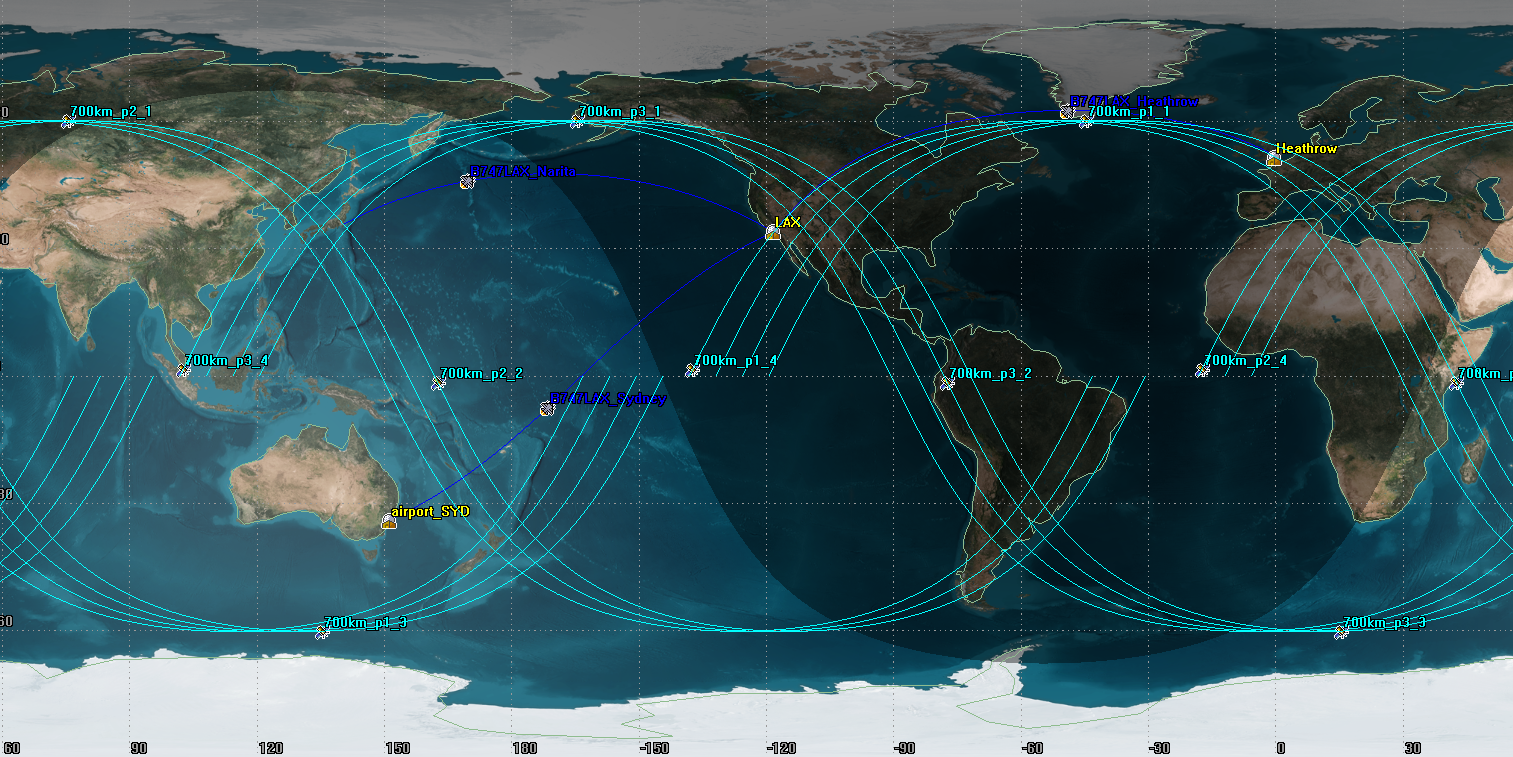
\includegraphics[scale = 0.40]{Pictures/12sat_2d.png}
	
	\caption{Ground track of the 12 satellite reference configuration in STK}
	\label{fig:12sat_2d}
\end{figure} 

\begin{figure}[htbp]
	\centering
	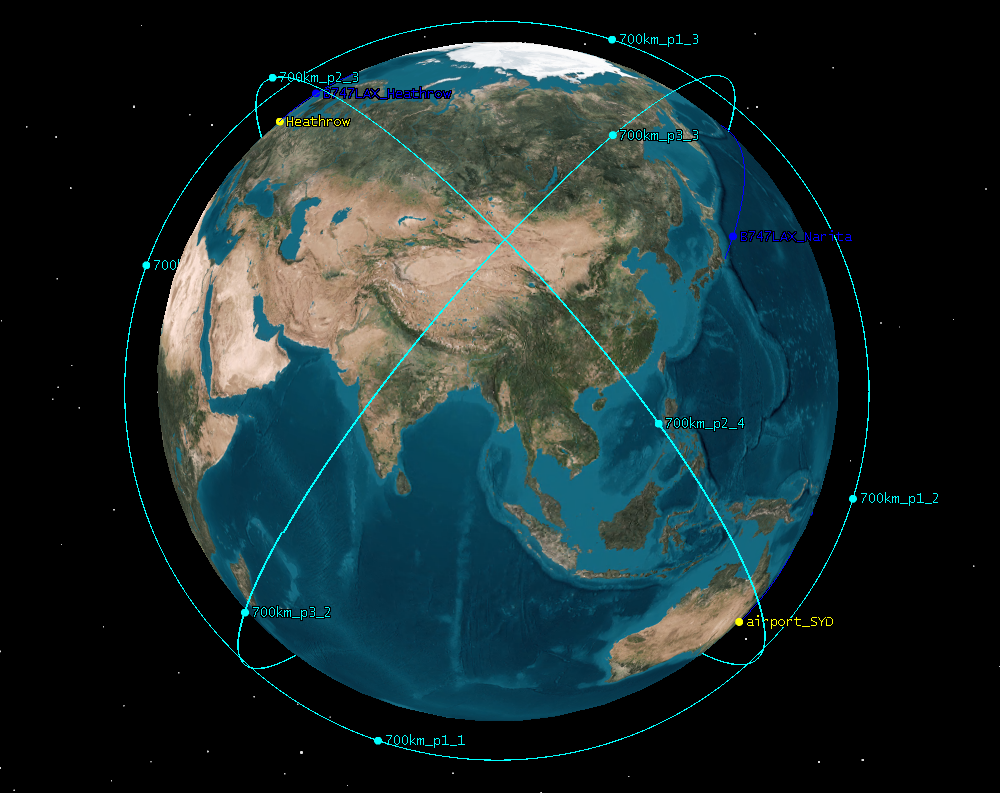
\includegraphics[scale = 0.4]{Pictures/12sat_3d.png}
	
	\caption{3D model of the 12 satellite reference configuration in STK}
	\label{fig:12sat_3d}
\end{figure} 

It was expected that change in inclination, altitude and number of satellites will effect the performance of a given constellation. An increase in altitude would result in an increase in orbital period, but would also increase the receiver footprint of a given satellite with a greater field of view. The change in inclination would vary the maximum and average coverage gap times as the ground traces intersect with the flight paths in different ways.  The change in the number of satellites would change the average and maximum ADS-B coverage gaps, but provide a trade-off with the number of satellites requiring production, maintenance and replacement.

\subsection{Test Cases}
\label{sec:sat_testcases}
From the reference case, inclination, altitude and number of satellites per-plane were varied according to the values presented in Table \ref{tab:satInputParams}. The full table of cases evaluated is given in Appendix \ref{app:all_parameters}.
\begin{table}[H]
  \centering
  \caption{Varying input parameters used for data and analysis}
    \begin{tabular}{lrrr}
    \toprule
    Input Parameter & Minimum & Maximum & Step Size \\
    \midrule
    Altitude & 400km & 800km & 50km  \\
    Satellites per plane & 1 & 6 & 1\\
    Inclination & 30$^\circ$ & 90$^\circ$ & 10$^\circ$ \\
    \bottomrule
    \end{tabular}%
  \label{tab:satInputParams}%
\end{table}%
\subsection{Analysis Period} \label{sec:analysis_period}
Synchronisation and periodicity were taken into account in selecting an analysis period. The discrepancy between air speed of planes (in the order of 250m/s) and the orbital velocity of LEO satellites (in the order of 8km/s) resulted in asynchronous behaviour.  The analysis period was therefore chosen to be long enough to such that - 
\begin{itemize}
	\item The effective ground track for one satellite would form a continuous swath between the latitudes of inclination. The length of period was chosen so that the ground track would repeat over the same global co-ordinates at least once. 
	\item The aggregate results of analysis would accurately take into account all cases where the lack of synchronisation between orbital period and flight time would produce abnormal results. That is, sufficiently many orbital and flight periods are repeated in order to observe an accurate aggregate effect and identify each of the worst-case scenarios.
\end{itemize} 
After initial tests it was found that an analysis period of approximately six days was appropriate. In STK the scenario was analysed between 12:00AM on December 6th, 2013 to 12:00AM December 9th, 2013, $\pm$ 24 hours to allow for varying flight times.
